\documentclass[12pt,letterpaper]{exam}
%\usepackage{color}
\usepackage[usenames,dvipsnames,svgnames,table]{xcolor}
\usepackage[margin=0.9in]{geometry}
\renewcommand{\familydefault}{\sfdefault}
\usepackage{multicol}
\pagestyle{head}
\definecolor{c03}{HTML}{FFDDDD}
\header{AM 108 Problem Set 05}{Updated on \today.}{{\colorbox{c03}{\makebox[3.0cm][l]{Due Fri Mar 8}}}\\ at noon}
\runningheadrule
\headrule
\usepackage{diagbox}
\usepackage{graphicx} % more modern
%\usepackage{subfigure} 
\usepackage{amsmath} 
\usepackage{amssymb} 
%\usepackage{gensymb} 
%\usepackage{natbib}
\usepackage{hyperref}
%\usepackage{enumitem}
%\setlength{\parindent}{0pt}
%\usepackage{setspace}
%\pagestyle{empty}  
%\newcommand{\Sc}[0]{
%{\color{BlueViolet}\S}
%}
\usepackage{tcolorbox}
\usepackage[framed,numbered,autolinebreaks,useliterate]{mcode}

\begin{document}
 \pdfpageheight 11in 
  \pdfpagewidth 8.5in


\begin{questions}
\question Consider the system 
\begin{align*}
\dot{x} &= -\mu y + x y\\
\dot{y} &= \mu x + \frac{1}{2}(x^2-y^2).
\end{align*}
\begin{parts}
\part In the class activity from Class 11, you may have shown that the fixed points are $(0,0)$, $(-2\mu,0)$, $(\mu, \sqrt{3}\mu)$ and $(\mu, -\sqrt{3}\mu)$.  You may have also classified these in their respective linearized systems (linear center, saddle, saddle, saddle), and shown that the system has a conserved quantity, $H(x,y)$.  

Find the conserved quantity, showing your steps.  % \emph{You can check your work on this against the solution from the class activity.}

\part Find $H(x,y)$ at each of the fixed points.


\part Show that the line $x = \mu$ is an invariant of this system.

An invariant of a dynamical system is a set of points such that, if you start at a point within the set, you'll stay within the set for all time (forwards and backwards).  One example of a (somewhat trivial) invariant set is a fixed point.  If you start at the fixed point you stay there for all time.  A second example of a (trivial) invariant set is the whole phase space: whatever your initial conditions within the phase space, you'll stay within the phase space for all time.


%Note that this line passes through two of the fixed points, so $H(x,y) = c$ where at all points $(x,y)$ on the line $x = \mu$, where $c$ is the value of $H(x,y)$ at the fixed points.
\part There are two other invariant lines and they intersect the $x=\mu$ line.  Find these lines.

\emph{Here's one procedure for this:}
\begin{itemize}
\item  Since the lines intersect the $x=\mu$ line we know that the lines are in the set of points where $H(x,y) = H(\mu,y) = c$.  So the points on the line $x=\mu$, and on the new lines, satisfy $H(x,y) - c = 0$.  This of this as a polynomial equation where you know $x-\mu = 0$ is one possible solution.  You can divide $(x-\mu)$ into $H(x,y) - c$ to factor the polynomial into $(x-\mu)K(x,y) = 0$.  The other two lines must be roots of $K(x,y) = 0$.  If you finds solutions of the form $y = ...$ based on the expression $K(x,y) = 0$, you'll find the other two lines.

\item For more info on this process, see \url{https://en.wikipedia.org/wiki/Synthetic_division}
\end{itemize}



\part Using the invariant lines you found above, along with local fixed point information and the vector field, sketch a phase portrait for the system.  Your sketch doesn't need to be correct, it just needs to be consistent with the vector field, the invariant lines, and the locally linear information you have for each fixed point.

\begin{solution}

The invariant line $x = \mu$ intersects $ y = \frac{1}{\sqrt{3}}(x+2\mu)$ at $(\mu,\sqrt{3}\mu)$ and intersects $y = \frac{1}{\sqrt{3}}(x+2\mu)$ at $(\mu, -\sqrt{3})$, so I can draw these onto my phase portrait.

Along $x = \mu$, $\dot y = \mu^2 + \frac{1}{2}(\mu^2 - y^2) = \frac{1}{2}(3\mu^2 - y^2)$.  This is negative for $\vert y\vert > \vert \mu \vert$ and positive for $\vert y\vert < \vert \mu \vert$, so I can add time arrows to the invariant line $ x= \mu$.

The fixed points were already classified.  For the saddle points, I'll head to Mathematica to 
learn about the eigenvalues and eigenvectors.  

\begin{verbatim}
Clear[f, g, jacobian]
f[x_, y_] := y (-\[Mu] + x)
g[x_, y_] := \[Mu] x + (x^2 - y^2)/2
solns = Solve[{f[x, y] == 0, g[x, y] == 0}, {x, y}]
jacobian = {{D[f[x, y], x], D[f[x, y], y]}, {D[g[x, y], x], 
   D[g[x, y], y]}}
Tr[jacobian] /. solns
Det[jacobian] /. solns
Simplify[Eigensystem[jacobian] /. solns]
\end{verbatim}


For $(\mu, \sqrt{3}\mu)$ I find the stable direction is $[0; 1]$ and the unstable direction is $[\sqrt{3}; 1]$.  The invariant lines are the stable and unstable manifolds of the saddle points.  Using $(\mu, \sqrt{3}\mu)$ to set the arrow directions, and knowing that we have a nonlinear center at $(0,0)$, I fill in a phase portrait:

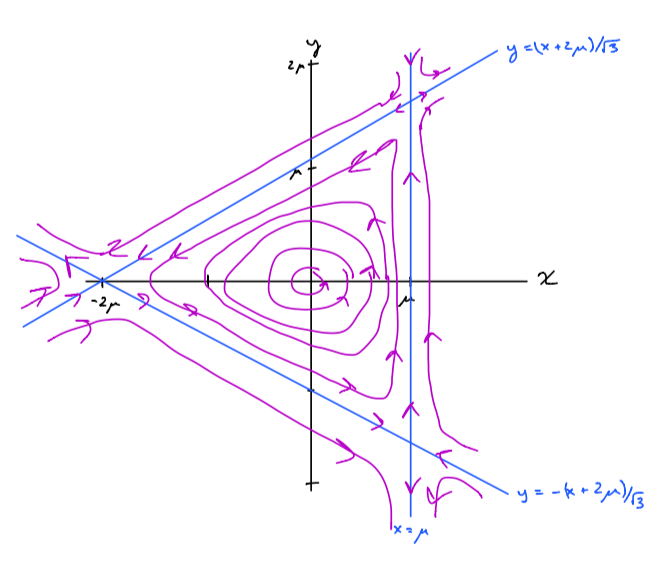
\includegraphics[width=4in]{img/Pset05q1e.png}

% I'll classify the fixed points as well: $f_x = y$, $f_y = x - \mu$, $g_x = \mu + x$, $g_y = -y$.  The trace is $y - y = 0$ and the determinant is $y(-y) - (\mu + x)(x-\mu) = -y^2 - x^2 + \mu^2$. Classifying the fixed points:

% \begin{tabular}{ c | c | c}
% fixed point & determinant \\
% \hline 
% \hline
% $(0,0)$ &  $\mu^2$ & linear center \\
% \hline
% $(-2\mu, 0)$ & $-3\mu^2$ & saddle point \\
% \hline
% $(\mu, \sqrt{3}\mu)$ & $<0$ & saddle point \\
% \hline
% $(\mu, -\sqrt{3}\mu)$ & $< 0$ & saddle point
% \end{tabular}

% For each saddle point, I'll head to Mathematica to find eigenvalues and eigenvectors.

\end{solution}


\part Identify any heteroclinic or homoclinic connections in your system.

\begin{solution}

The invariant lines connect saddle points so the segments of the invariant lines that connect that saddles are heteroclinic orbits.  There are three of these.

\end{solution}

\part Use a numerical tool to create an accurate phase portrait (include the name of the tool and any code or instructions needed to reproduce your plot).


\begin{solution}

To make the phase portrait, I use StreamPlot in Mathematica.  I added the fixed points to the portrait and made an additional StreamPlot choosing initial conditions right on the heteroclinic connections so that those are visible in the plot.

\begin{verbatim}
f[x_, y_] := y (-\[Mu] + x)
g[x_, y_] := \[Mu] x + (x^2 - y^2)/2
solns = Solve[{f[x, y] == 0, g[x, y] == 0}, {x, y}]
fixed = ListPlot[{x, y} /. solns /. \[Mu] -> 3, AspectRatio -> 1, 
  PlotMarkers -> Graphics[{Black, Thick, Circle[]}, ImageSize -> 10], 
  Ticks -> {{{-3, -\[Mu]}, {3, \[Mu]}}, {{-3, -\[Mu]}, {3, \[Mu]}}}, 
  AxesLabel -> {x, y}, LabelStyle -> Medium, 
  PlotRange -> {{-8, 4}, {-6, 6}}]
val = 7;
sp = StreamPlot[({f[x, y], g[x, y]} /. \[Mu] -> 3), {x, -val, 
    val}, {y, -val, val}, Frame -> False];
sp1 = StreamPlot[({f[x, y], g[x, y]} /. \[Mu] -> 3), {x, -val, 
   val}, {y, -val, val}, 
  StreamPoints -> {{3, 0}, {0, 2 Sqrt[3]}, {0, -2 Sqrt[3]}}];
Show[fixed, sp, sp1]
\end{verbatim}

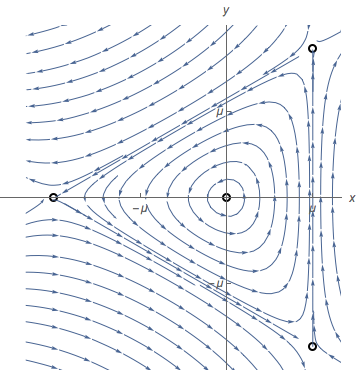
\includegraphics[width=4in]{img/S19pset05p2.png}

\end{solution}

\end{parts}

\question (Projects) This assignment is related to option 2 of the project types (see ``Extra Information'' below).
\begin{itemize}
    \item Do a search for a published paper that relates to dynamical systems or bifurcation theory and connects to a topic you are interested in.  Read the abstract to the paper.  
    
    Each student should find a unique paper for this, so check the Piazza posts: if the paper you found has already been posted about to Piazza, search for a different paper on which to base your post.
    \item In addition, choose one of the papers from the Reference list in this problem set, search for that paper, and read the abstract.
    
    This one doesn't need to be unique.  You can post about the same abstract as other another student.
    
    \item Add a followup post in the Pset 05 Project thread on Piazza.  Either start a new followup (if no other posts are on similar topics to the one you chose) or post within a followup started by another student (if the paper you found is on a related topic).  In your post, give the title, authors, and year of each of the two papers, and make a brief comment about each abstract.  You might mention something you found interesting, something you didn't understand, or anything else that seems worth sharing.
\end{itemize}  

To do the searches, you might use \url{https://scholar.google.com} or another scientific index.  If you use an index beside Google Scholar, mention it in your post.  

Search terms related to our course could include \emph{bifurcation, stability, dynamical} etc.  To look up a specific paper, typing in the title of a paper is a good way to find it.

If you would like to access the full text of the paper, go to \url{https://hollis.harvard.edu} and enter the title of the paper in the search bar there.  This is a Harvard library website and will give you access to the paper if Harvard has a subscription.  If not, it usually has a link for requesting the paper via BorrowDirect / Interlibrary Loan.

\textbf{Extra information}

There will be three options for the structure of your project:
\begin{enumerate}
    \item It can be a dynamical systems modeling project.  In that case, you would work to build a dynamical model (likely a very simple model) with the aim of answering a question you're intrigued by.
    \item It can be based on a paper.  In that case, you would work to understand the key results and would add an extension or new exploration.  Your contribution requires an act of creative ownership: you might adjust some aspect of the model, shift it to a different context, explore a special case, or anything else you propose.  I will provide a list of possible papers for this (\emph{see attached list}), or you can propose a paper.  Only one team per paper.
    \item It can be learning-oriented with a focus on exploring a dynamical systems topic that is beyond the scope of our course.  In that case, you'll learn about the topic and then will develop materials to guide your classmates or future students in learning about the topic.  A few suggested topics are listed in the ``Exploration Topics'' section.
\end{enumerate}


We will spend some time in class on \textbf{Friday March 8th} splitting apart by potential interest area so that students with economics / biology / climate / social systems / etc project interests can meet each other.


The default for the project will be to work in a student-selected team of three.  If there's a reason that a group of one, two, or four would work better, you'll have a chance to speak with me about arranging an exception. 

The project proposals will be due \textbf{Monday, April 1st}.  A timeline for the project deliverables and more detailed expectations will be included in problem set 06.

\textbf{Potential exploration topics}
\begin{itemize}
    \item pattern formation (Turing bifurcation)
    \item spatially extended systems
    \item fast-slow systems
    \item Melnikov method and routes to chaos
    \item noise (stochasticity) in dynamical systems
    \item data assimilation
    \item control of a dynamical system
    \item equation-free methods
\end{itemize}

\nocite{*}
\bibliographystyle{plain}
\bibliography{projects}

% \begin{itemize}
%     \item \textbf{Monday, April 1}: Project proposals due.
%     \begin{itemize}
%         \item If you're basing your project on a paper from the list I've provided, you'll send me a message on Piazza letting me know the paper once you've chosen it, along with the names of your team members, so that I can update the set of available titles.
%     \end{itemize}
%     \item \textbf{Mondays in April}; Project updates.  A project update, along with a team meeting log, an updated reference list, and any simulation code, will be due the 8th, 15th, and 22nd of April.
%     \item \textbf{Friday, April 26}: Peer-editing 1: Presentation.  A draft of your presentation will be due Thursday April 25th.
%     \item \textbf{Monday, April 29 + Wednesday, May 1}: Project presentation 1.
%     \item \textbf{Wednesday, May 1}: Project presentation 1.
%     \item \textbf{Friday, May 3}: Peer-editing 2: 
%     \item \textbf{Saturday, May 11}: Project presentation 2 + Final report.
    
% \end{itemize}

% \noindent The project will consist of two parts: a 10-15 page paper, and a $7$ minute presentation.
%  \vskip.25in

% \noindent
% {\bf The paper:}~(45\% of project grade) The purpose of this part of the project is to practice and refine your written mathematical communication skills that you have been cultivating on homework assignments throughout the semester. This paper should be (roughly) between 10 and 15 pages long, typed in LaTeX, and aimed at an audience of your peers. IMPORTANT: your paper should NOT simply be a rewording or restating of the paper you are studying. You should introduce the background, summarize the authors' key results {\em in your own words}, and then explain your extensions or new results. You should cite any relevant work. You can assume the reader understands everything that we have learned in this class, but you shouldn't assume further mathematical or physical knowledge. Your paper should be in the style of a mathematical document; that is, you should define all new objects you introduce, state and explain models precisely, and give examples. You will be provided with a LaTeX template (link on Piazza) to help you get started. If you are still unclear about what style I am expecting for this document, come talk to me. This document is your magnum opus of the semester. Take time to create something that illustrates your newly obtained knowledge/skillset and is a manuscript you can be proud of. Also - edit this! Several times! Grading rubric is attached.
% \vskip.25in
% \noindent
% {\bf The presentation:}~(45\% of project grade) The purpose of this part of the project is to demonstrate your verbal mathematics communication skills that you have been developing by working with your peers in class. Each group will give a $7$ minute presentation on their project. Groups may decide to have one person give the presentation, or multiple group members may split the presentation time. Be aware that seven minutes is not very long to explain a 10-15 page paper! This means you should practice to make sure you fall within the allotted time. Think carefully about what you are going to say and how you can best express your ideas concisely. You are welcome to use either presentation tools (Powerpoint, Beamer slides, etc.) or just boards. Grading rubric is attached.
% \vskip.25in
% \noindent
% Finally, if you have no idea what to do your project on or who to work with, come talk to me! I'm here to help you and make this a positive experience - please reach out to me if the idea of this project is making you anxious. 



\end{questions}




\end{document}
